\input{/home/nick/latex-preambles/xelatex.tex}

\newcommand{\imagesPath}{.}

\title{
	\textbf{Δίκτυα Υπολογιστών} \\~\\
	Εργαστηριακή Άσκηση 5 \\ 
	Εξερεύνηση του Διαδικτύου
}
\author{}
\date{}

\begin{document}
	\maketitle
	
	\begin{tabular}{|l|l|}
		\hline
		\textbf{Ονοματεπώνυμο:} Νικόλαος Παγώνας, el18175 & \textbf{Ομάδα:} 4 (Τρίτη εξ' αποστάσεως) \\
		\hline
		\textbf{Όνομα PC/ΛΣ:} nick-ubuntu/Ubuntu 20.04.3 LTS & \textbf{Ημερομηνία:} Τρίτη 09/11/2021  \\
		\hline
		\textbf{Διεύθυνση IP:} \verb|192.168.1.15| & \textbf{Διεύθυνση MAC:} \verb|3c:2c:30:e1:1c:55|\\
		\hline
	\end{tabular}

	\section*{1 - Ο χρόνος ζωής των πακέτων IPv4}
		\subsection*{1.1}
			Η διεύθυνση της εικονικής διεπαφής tun0 είναι 147.102.131.182.
		
		\subsection*{1.2}
			Η μάσκα υποδικτύου είναι 255.255.255.0, οπότε το μήκος προθέματος δικτύου είναι 3 bytes.
		
		\subsection*{1.3}
			Η σύνταξη της εντολής είναι \verb|ping -c 1 -t <TTL> <IP Address>|.
		
		\subsection*{1.4}
			Η ελάχιστη τιμή για να φτάσει το πακέτο στο 176.126.38.1 είναι TTL = 3.
		
		\subsection*{1.5} 		
			\begin{figure}[H]
				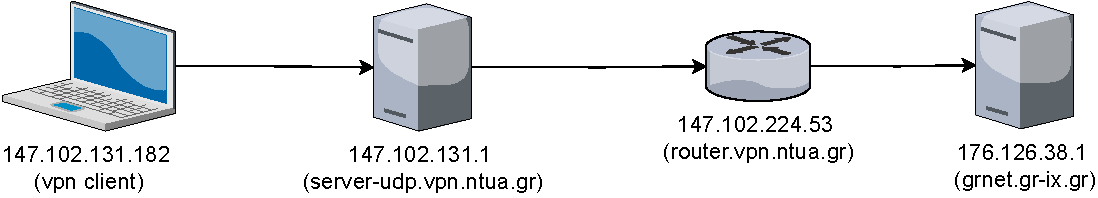
\includegraphics[width=\linewidth]{\imagesPath/1.5.pdf}
			\end{figure}
			
	\section*{2 - Ανακαλύψτε την τοπολογία}
		\subsection*{2.1}
			Αν χρησιμοποιήσουμε UDP datagrams έχουμε συνεχόμενες εκπνοές χρόνου, οπότε με το flag -I στέλνουμε ICMP πακέτα για να μπορέσουμε να συνεχίσουμε την άσκηση. \\
			Έτσι, η σύνταξη της εντολής είναι: \\~\\ 
			\verb|traceroute -4 -I www.ntua.gr| \\~\\
			Παρατηρούμε ότι τόσο η διαδρομή, όσο και τα CNAMEs είναι διαφορετικά σε σχέση με το παρελθόν.
			
		
		\subsection*{2.2}
			Επειδή με UDP και ICMP είχαμε παρόμοιο θέμα με το προηγούμενο ερώτημα, χρησιμοποίησαμε το πρωτόκολλο TCP.
			
			\begin{figure}[H]
				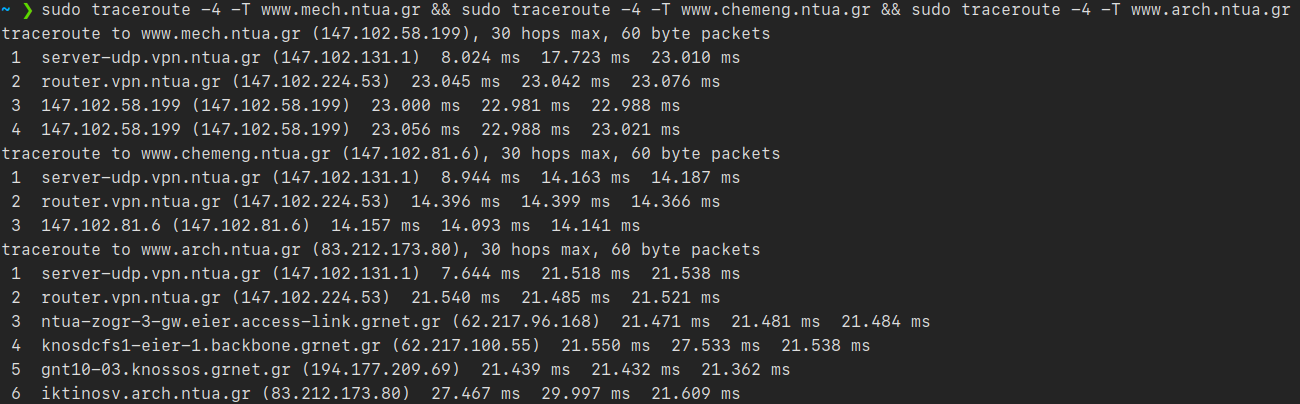
\includegraphics[width=\linewidth]{\imagesPath/2.2.png}
			\end{figure}
		
			\begin{figure}[H]
				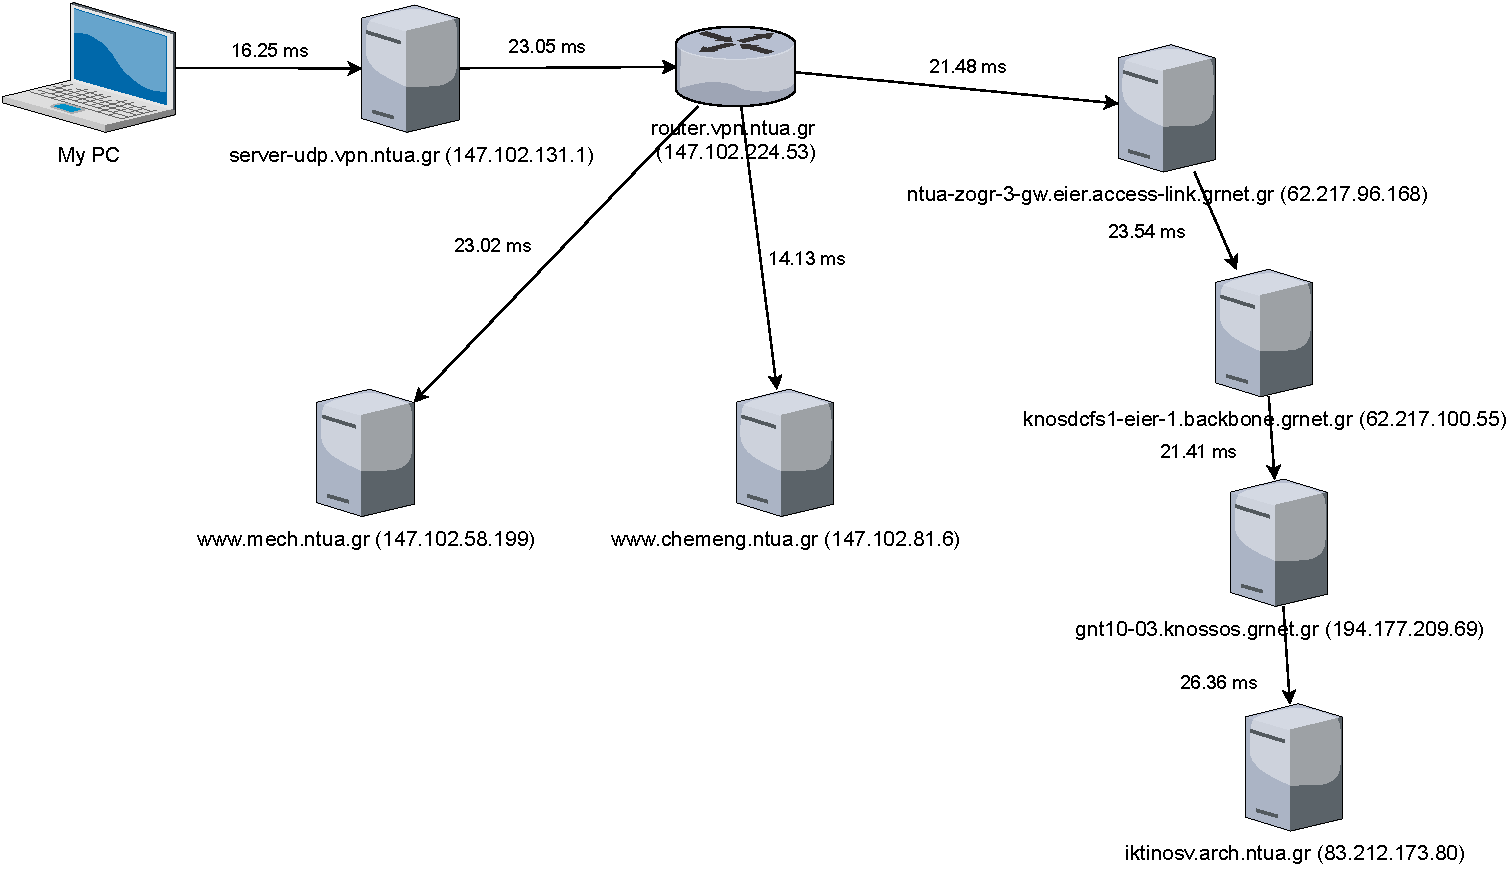
\includegraphics[width=\linewidth]{\imagesPath/2.2.pdf}
			\end{figure}
			
		\subsection*{2.3}
			Ναι, συμφωνεί σε μεγάλο βαθμό, απλώς δεν μπορούμε να βρούμε τα switches με την παραπάνω μέθοδο.
		
		\subsection*{2.4}
			Η σύνταξη της εντολής που χρησιμοποιήσαμε είναι: \\~\\
			\verb|traceroute -4 -m 4 <IP Address>|
		
		\subsection*{2.5}
			\begin{figure}[H]
				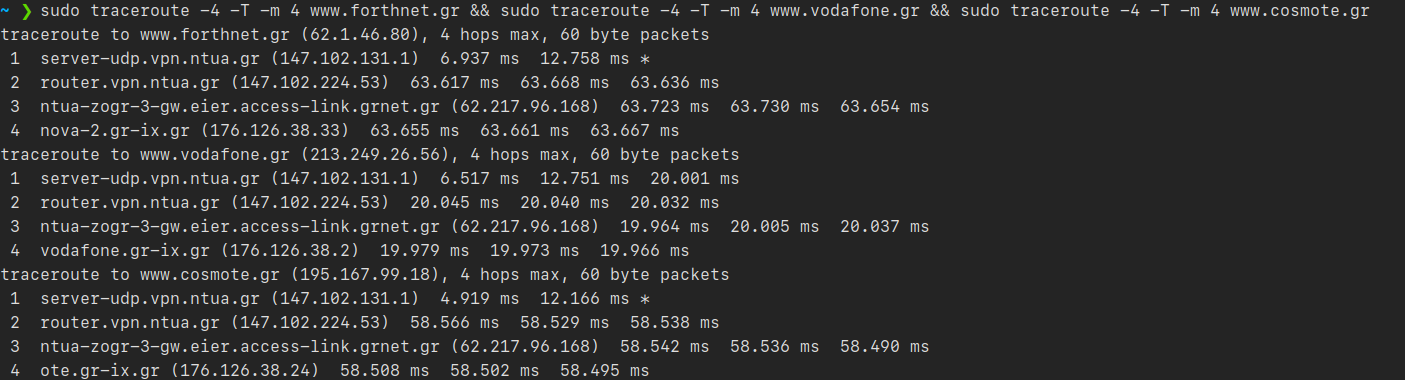
\includegraphics[width=\linewidth]{\imagesPath/2.5.png}
			\end{figure}
		
			\begin{figure}[H]
				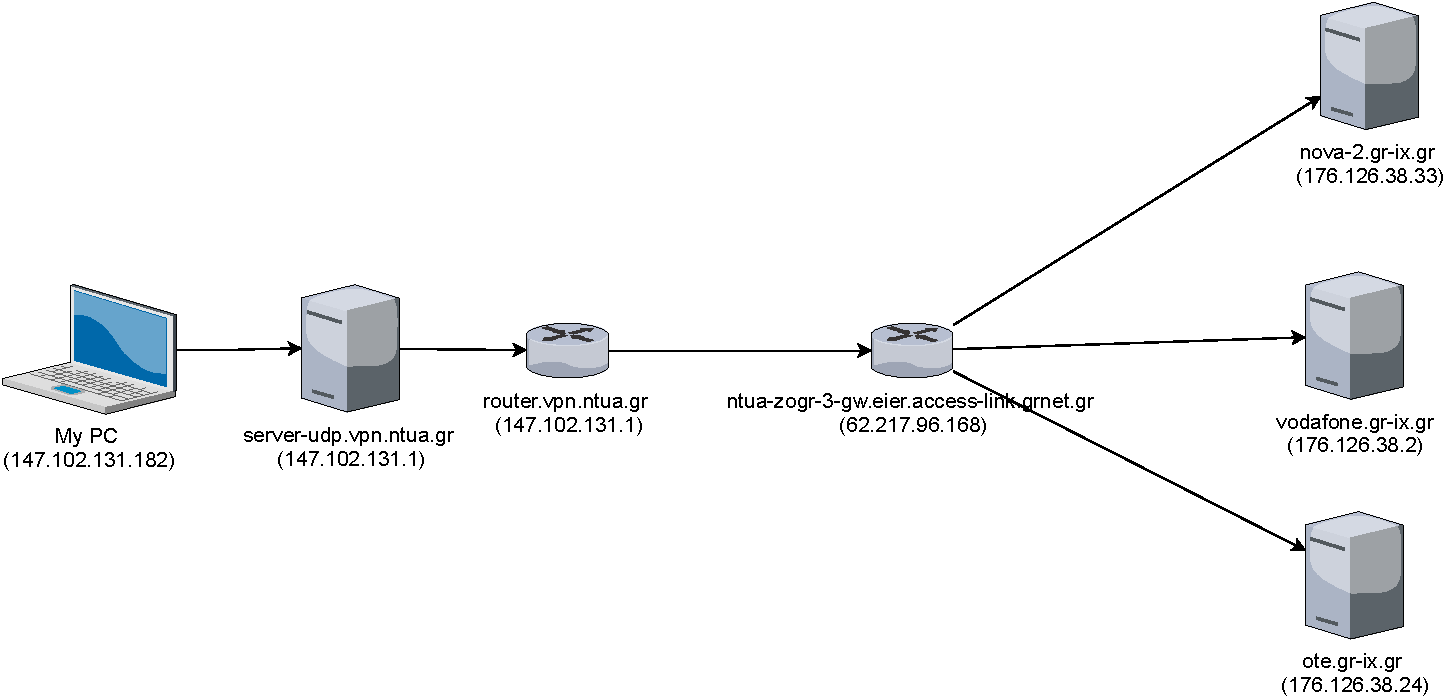
\includegraphics[width=\linewidth]{\imagesPath/2.5.pdf}
			\end{figure}
		
		\subsection*{2.6}
			Ναι συμφωνεί σε αρκετά μεγάλο βαθμό.
		
		\subsection*{2.7}
			Η διεύθυνση υποδικτύου του GR-IX είναι 176.126.38.0/24.
		
		\subsection*{2.8}
			Η σύνταξη της εντολής traceroute που χρησιμοποιήσαμε είναι: \\~\\
			\verb|traceroute -4 -In grnet.gr-ix.gr|
		
		\subsection*{2.9}
			Η σύνταξη του φίλτρου απεικόνισης που χρησιμοποιήσαμε είναι \verb|icmp|.
		
		\subsection*{2.10}
			Η τιμή του πεδίου Protocol είναι 0x01 (ICMP).
		
		\subsection*{2.11}
			Σύμφωνα με το Wireshark, έχουμε total length 60 bytes, header length 20 bytes, άρα το πακέτο μεταφέρει 40 bytes στο πεδίο δεδομένων.
		
		\subsection*{2.12}
			Αποστέλλονται και λαμβάνονται 3 τριάδες.
		
		\subsection*{2.13}
			\begin{tabular}{|c|c|c|}
				\hline
				\textbf{TTL} & \textbf{Παραλήπτης μηνύματος} & \textbf{Διεύθυνση από όπου έρχεται η απάντηση} \\
				\hline
				1 & 176.126.38.1 & 147.102.131.1 \\
				\hline
				2 & 176.126.38.1 & 147.102.224.53 \\
				\hline
				3 & 176.126.38.1 & 176.126.38.1 \\
				\hline
			\end{tabular}
		
		\subsection*{2.14}
			Ναι, οι διευθύνσεις είναι οι ίδιες.
		
		\subsection*{2.15}
			Για την πρώτη τριάδα έχουμε TTL = 1, για την δεύτερη TTL = 2 και για την τρίτη TTL = 3.
		
		\subsection*{2.16}
			Για την πρώτη τριάδα έχουμε TTL = 64, για την δεύτερη TTL = 254 και για την τρίτη TTL = 62.
		
		\subsection*{2.17}
			Γιατί τα πρώτα πακέτα που έχουν μικρό TTL φτάνουν στους πρώτους κόμβους, οι οποίοι βλέπουν το (πλέον μειωμένα) TTL να έχει γίνει ίσο με 0, και έτσι απαντούν στον αποστολέα με Time-to-live exceeded. 
		
		\subsection*{2.18}	
			Ο προορισμός απαντά με Echo (ping) reply. 
	

	\section*{3 - Περισσότερα για τις επικεφαλίδες πακέτων IP}
		\subsection*{3.1}
			Η σύνταξη της εντολής που χρησιμοποιήσαμε είναι \verb|traceroute -4 -I nic.gr-ix.gr|

		\subsection*{3.2}
			Το φίλτρο σύλληψης που χρησιμοποιήσαμε είναι \verb|icmp|.

		\subsection*{3.3}
			\begin{figure}[H]
				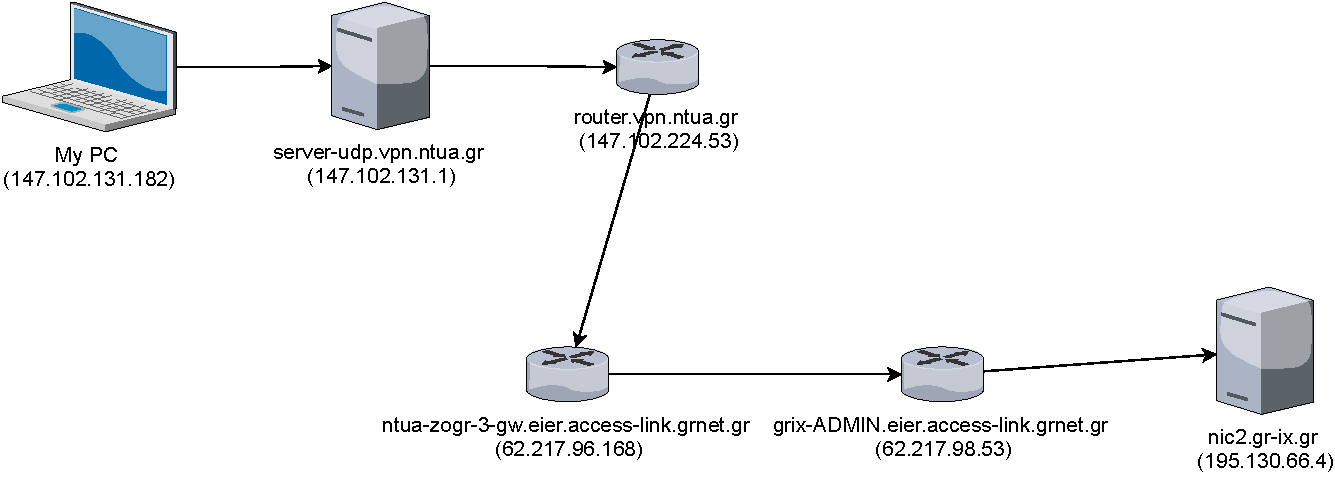
\includegraphics[width=\linewidth]{\imagesPath/3.3.pdf}
			\end{figure}

		\subsection*{3.4}
			Αλλάζουν τα πεδία Identification, TTL και Header Checksum.
		
		\subsection*{3.5}
			Τα πεδία που παραμένουν αμετάβλητα σε όλη την σειρά είναι όλα τα υπόλοιπα.

		\subsection*{3.6}
		
			Τα πεδία που πρέπει να παραμείνουν αμετάβλητα είναι:
			\begin{itemize}
				\item \textbf{Version:} Γιατί έχουμε ζητήσει να είναι Version 4.
				\item \textbf{Total Length:} Γιατί στέλνουμε το default μέγεθος.
				\item \textbf{Protocol:} Γιατί έχουμε ICMP λόγω του flag -Ι.
				\item \textbf{Source Address:} Έχει οριστεί από εμάς.
				\item \textbf{Destination Address:} Επίσης έχει οριστεί από εμάς.
			\end{itemize}
		
		\subsection*{3.7}
			Τα πεδία που πρέπει να αλλάξουν είναι:
			\begin{itemize}
				\item \textbf{Identification}: Διότι δεν έχουμε fragmentation.
				\item \textbf{TTL}: Λόγω της λειτουργίας της εντολής traceroute (σταδιακή αύξηση του TTL)
				\item \textbf{Header Checksum}: Αφού έχουμε πεδία που αλλάζουν, άρα και το Checksum θα είναι διαφορετικό.
			\end{itemize}
			
		\subsection*{3.8}
			Η τιμή του TTL του πρώτου πακέτου της σειράς ICMP Time Exceeded είναι 64.

		\subsection*{3.9}
			Ναι, γιατί αυτή η σειρά αποτελεί την απάντηση σε τρία πακέτα ICMP, τα οποία είχαν το ίδιο TTL όταν έφυγαν.

		\subsection*{3.10}
			Έχουμε TTL = 254.

		\subsection*{3.11}
			TTL = 60.

		\subsection*{3.12}
			TTL = 64, αφού έχουμε 4 hops μέχρι να φτάσουν στον υπολογιστή μας.

	\section*{4 - IPv4 options}
		\subsection*{4.1}
			Η σύνταξη της εντολής ping είναι: \verb|ping -4 -c 1 -R www.ntua.gr|.

		\subsection*{4.2}
			Η επικεφαλίδα του πακέτου που έστειλε ο υπολογιστής μας έχει μέγεθος 60 bytes.

		\subsection*{4.3}
			Η επικεφαλίδα του πακέτου που έλαβε ο υπολογιστής μας έχει μέγεθος επίσης 60 bytes.

		\subsection*{4.4}
			Το πεδίο Options έχει μήκος 40 bytes (επειδή ζητήσαμε να ενεργοποιηθεί η καταγραφή διαδρομής), εξού και το αυξημένο μέγεθος.

		\subsection*{4.5}
			\begin{figure}[H]
				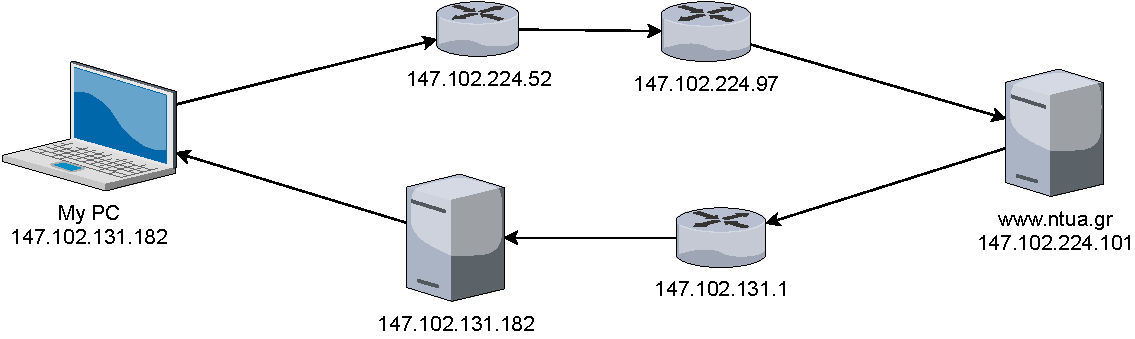
\includegraphics[width=\linewidth]{\imagesPath/4.5.pdf}
			\end{figure}		

		\subsection*{4.6}
			Η διεύθυνση του nic.grnet.gr είναι 194.177.210.210, και βρίσκεται 5 βήματα μακριά.

		\subsection*{4.7}
			\begin{enumerate}
				\item server-udp.vpn.ntua.gr (147.102.131.1) 
				\item router.vpn.ntua.gr (147.102.224.53)  
				\item ntua-zogr-3-gw.eier.access-link.grnet.gr (62.217.96.168)
				\item kolettir-eier-AE.backbone.grnet.gr (62.217.100.62)
				\item pdns1.grnet.gr (194.177.210.210) 
			\end{enumerate}
			

		\subsection*{4.8}
			\begin{enumerate}
				\item vpn2.noc.ntua.gr (147.102.224.52)
				\item ntua-zogr-3.eier.access-link.grnet.gr (62.217.96.169)
				\item eier-kolettir-AE.backbone.grnet.gr (62.217.100.63)
				\item koletti-serverlan-gw.grnet.gr (194.177.210.193)
				\item pdns1.grnet.gr (194.177.210.210)
			\end{enumerate}

		\subsection*{4.9}
			\begin{figure}[H]
				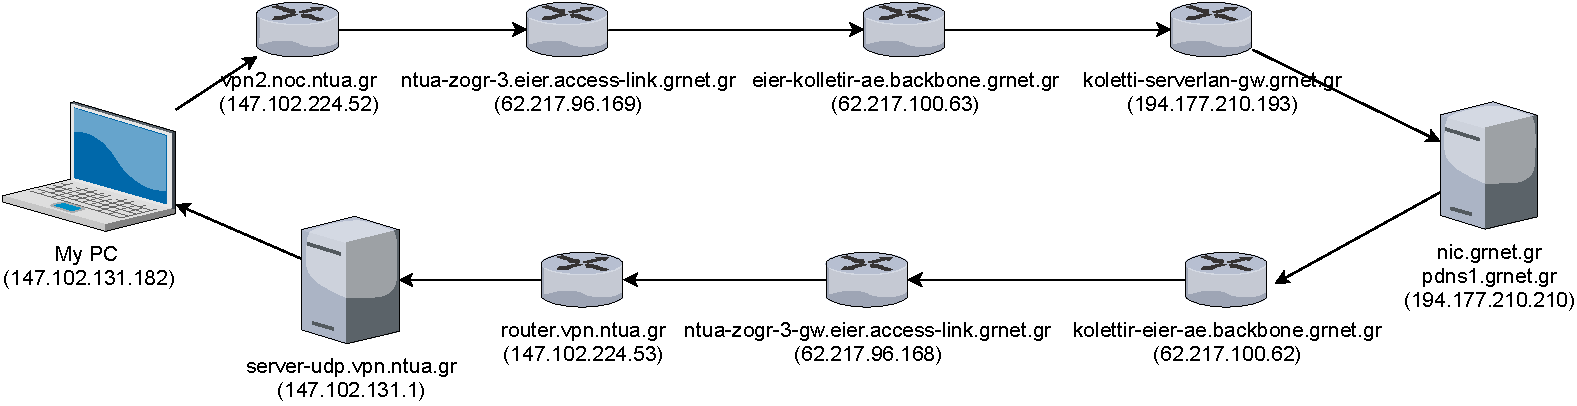
\includegraphics[width=\linewidth]{\imagesPath/4.9.pdf}
			\end{figure}
\end{document}